\part{Software Process}

\chapter{Software Development Lifecycle}\label{software-development.chapter}

This chapter describes the software development lifecycle (SDLC) for
Stan, RStan, CmdStan, and PyStan. The layout and content very closely
follow the R regularoty compliance and validation document
\citep[Section~6]{RProject:2014}.

\section{Operational Overview}

The development, release, and maintenance of Stan is a collaborative
process involving the Stan development team.  The team covers multiple
statistical and computational disciplines and its members are based at
both academic insitutions and industrial labs.

Communication among team members takes place in several venues.  Most
discussions take place openly on the Stan developers group, often
initiated by discussions in the Stan users group.%
%
\footnote{The groups are hosted by Google Groups, with information on
  reading and posting available from \url{http://mc-stan.org/groups.html}.}
%
The users and developers groups are archived and may be read by
anyone at any time. Communication that's not suitable for the public,
such as grant funding, is carried out on a private group restricted to
the core Stan developers. Further issue-specific discussion takes
place concurrently with development and source control.%
%
\footnote{The issue tracker for feature requests and bug reports is
  hosted by GitHub.  Full information on reading and making issue
  reques4ts is available from \url{http://mc-stan.org/issues.html}.}
%
Bigger design issues and discussions that should be preserved take
place on the project Wiki.%
%
\footnote{The Wiki is hosted by GitHub; see
  \url{https://github.com/stan-dev/stan/wiki}.}

The developers host a weekly videoconference during which project
issues are discussed and prioritized.%
%
\footnote{The weekly meetings are hosted on Google+.  They are not
  recorded or stored.}
%
The developers also meet informally at their places of employment
(e.g., Columbia University) or at conferences and workshops when
multiple team members are in attendance.  The developers also host
meetups for the public in locations including London and New York.%
%
\footnote{These meetings are organized through
  \url{http://meetups.com}.  For example, meetings in New York are
  organized through \url{http://www.meetup.com/Stan-Users-NYC/}.}

The Stan project employs standard software development, code review,
and testing methododologies, as described on the project Wiki pages
and later in this chapter.

Stan's C++ library and the CmdStan interface are released under the
terms of the new (3 clause) BSD license, with two dependent libraries
(Boost and Eigen), released under compatible libraries. The R
interface RStan and Python interface PyStan are released under the
GPLv3 license. All of the code is hosted on public version control
repositories and may be reviewed at any time by all members of the
Stan community.  This allows continuous feedback for both coding
standards, functionality, and statistical accuracy.

The size of the Stan community is difficult to estimate reliably
because there are no sales transactions and Stan's version control
distribution system (GitHub) does not provide download statistics.
There are over 950 users subscribed to the users group, and a
conservative estimate would put the number of users in the thousands.
This substantial user base provides the means to do continuous reviews
of real-world performance in real settings. Unlike proprietary
software only available in binary form, Stan's open-source code base
allows users to provide feedback at the code level.

\section{Source Code Management}

The source code for Stan's C++ library, CmdStan, PyStan, and RStan is
managed in separate version-control libraries based on Git
\citep{Chacon:2014} and hosted by GitHub under the GitHub organization
stan-dev (\url{https://github.com/stan-dev}). Push access (i.e., the
ability to write to the repository) is restricted to core developers
and very closely managed. At the same time, any user may provide (and
many users have provided) pull requests with patches for the system
(which are treated as any other pull request and fully tested and code
reviewed). Because of Git's distributed nature, everyone who clones a
repository produces a full backup of the system and all past versions.

\begin{figure}
\begin{center}
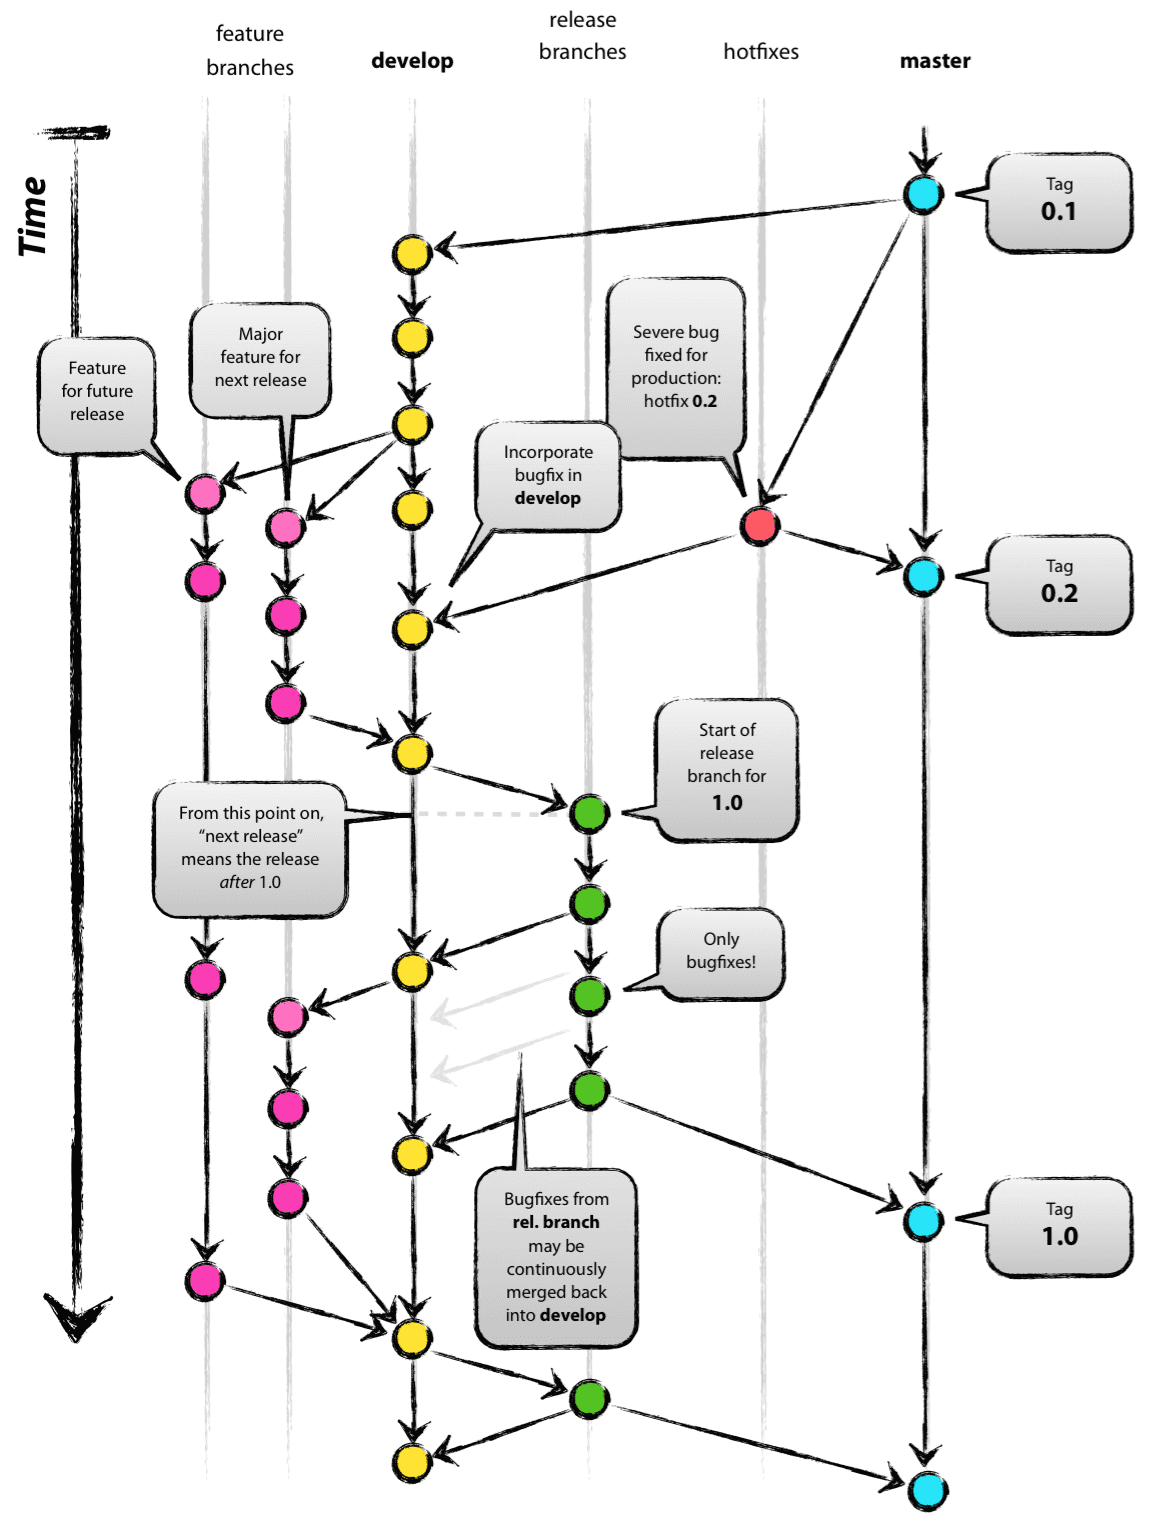
\includegraphics[height=4.5in]{img/git-process.png}
\end{center}
\caption{\small\it Git branching process for master
  and development branches.  New features and ordinary (not hot) 
  bugfixes are developed in branches from and merged back into the
  development  branch.  These are then
  collected into releases and merged with the master branch, which
  tracks the releases.  Hotfix branches are like feature or ordinary
  bugfix branches, but branch from master and merge back into master. 
  Image courtesy of \citep{Driessen:2010}.}\label{git-process.figure} \end{figure}
%
The basic Git process for branching, releasing, hotfixing, and merging
follows standard Git procedure \citep{Driessen:2010}. A diagram
outlining the process is presented in \reffigure{git-process}. The key
idea is that the master branch is always at the latest release, with
older commits tagged for previous releases. 

The development branch always represents the current state of
development. Feature and bugfix branches branch from the development
branch. Before being merged back into the development branch, they
must be wrapped in a pull request for GitHub, which supplies
differences with current code and a forum for code review and comment
on the issue. All branches must have appropriate unit tests and
documentation as part of their pull request before they will be merged
(see \url{https://github.com/stan-dev/stan/wiki/Pull-Request-Template}
for the pull request template which all requests must follow).  Each
pull request must provide a summary of the change, a detailed
description of the intended effect (often coupled with pointers to one
or more issues on the issue tracker and one or more Wiki pages), a
description of how the change was tested and its effects can be
verified, a description of any side effects, a description of any
user-facing documentation changes, and suggestions for reviewers.

Taken together, the testing, code review, and merge process ensures
that the development branch is always in a releasable state.

Git itself provides extensive log facilities for comparing changes
made in any given commit (which has a unique ID under Git) with any
other commit, including the current development or master branch.
GitHub provides further graphical facilities for commentary and
graphical differences.

For each release, the Git logs are scanned and a set of user-facing
release notes provided summarizing the changes. The full set of
changes, including differences with previous versions, is available
through Git.  These logs are complete back to the first version of
Stan, which was originally managed under the Subversion version
control system.

More information on the mechanics of the process are available from
on the Wiki page
\url{https://github.com/stan-dev/stan/wiki/Developer-Process}.

\section{Testing and Validation}

\subsection{Unit Testing}

Stan C++, CmdStan, PyStan, and RStan are all extensively unit tested.
The core C++ code and CmdStan code is tested directly in C++ using the
Google test framework \cite{GoogleTest:2011}. PyStan is tested using
the Python unit testing framework unittest%
%
\footnote{See \url{https://docs.python.org/3/library/unittest.html}.}
%
(formerly called ``PyTest'').  RStan is tested using the RUnit package.%
%
\footnote{See
  \url{http://cran.r-project.org/web/packages/RUnit/index.html}.}

The point of unit testing is to test the program ar the application
programmer interface (API) level, not the end-to-end functional level.  

The tests are run automatically when pull requests are created through
a continuous integration process. PyStan uses the Travis continuous
integration framework;%
%
\footnote{See \url{https://travis-ci.org} for more on Travis.}
%
Stan C++ and CmdStan use Jenkins.%
%
\footnote{See \url{http://jenkins-ci.org} for more on Jenkins.}
%
The continuous integration servers provide detailed reports of the
various tests they run and whether they succeeded or failed.  If they
failed, console output is available pointing to the failed tests.  The
continuous integration servers also provide graphs and charts
summarizing ongoing and past testing behavior.

Stan and its interfaces' unit tests are all distributed with the
system software and may be run by users on their specific platform
with their specific compilers and configurations to provide support
for the reliability of a particular installation of Stan.

As with any statistical software, users need to be careful to consider
the appropriateness of the statistical model, the ability to fit it
with existing data, and its suitability to its intended application.

The entire source repository is available to users.  A snapshot at any
given release (or commit within a branch) may be downloaded as an
archive (zip file) or may be cloned for development under Git.
Cloning in Git provides a complete copy of all version history,
including every commit to every branch since the beginning of the
project.  

User feedback is accomodated through three channels. First, and most
formally, there is an issue tracker for each of Stan C++, CmdStan,
RStan and PyStan, which allows users to submit formal bug reports or
make feature requests.  Any user bug report is reviewed by the
development team, assessed for validity and reproducibility, and
assigned to a specific developer for a particular release target.
A second route for reporting bugs is our users group;  bugs reported
to the user group by users are then submitted to the issue tracker by
the developers and then put through the usual process.  A third method
of bug reporting is informal e-mail or comments; like the user group
reports, these are channeled through the issue tracker by the
developers before being tackled.

Continuous integration is run on a combination of Windows, Mac OS X,
and Linux platforms.  All core Stan C++ code is tested on Windows, Mac
OS, and Linux before release.


\subsection{Functional Testing}

In addition to unit testing at the individual function level, Stan
undergores rigorous end-to-end testing of its model fitting
functionality. Models with known answers are evaluated for both speed
and accuracy. Models without analytic solutions are evaluated in terms
of MCMC error.  


\section{Release Cycles}

At various stages, typically when major new functionality has been
added or a serious bug has been fixed, the development branch is
declared ready for release by the Stan development team. At this
point, the branch is tested one last time on all platforms before
being merged with the master branch. Releases are managed through
GitHub releases mechanism.%
%
\footnote{For example, releases for Stan C++ are available on
\url{https://github.com/stan-dev/stan/releases}.}
%
Each release further bundles the manual and provides both a zipped and
tar-gzipped archive of the release.

Stan is released exclusively as source code, so nothing needs to be
done with respect to binary release management or compatibility.  The
source is tested so that it can be used under Windows, Mac OS X, and
Linux.  

Releases are numbered using a conventional major/minor/patch-level
scheme.  For example, version 2.0.0 is the first major release of
version 2 of Stan, whereas version 2.1.0 is the first minor feature
release of version 2 of Stan.  Version 2.1.1 would be used for a patch
that only fixes bugs in version 2.1.0 without adding any
functionality.  All numbers increment one at a time.

Instructions for installing Stan C++, CmdStan, RStan, and PyStan are
managed separately and distributed with the associated product.

\section{Availability of Current and Historical Archive Versions}

Current and older versions of Stan C++, CmdStan, RStan, and PyStan are
available through the GitHub pages for the corresponding repository.
Official releases are bundled as archives and available through
GitHub's releases (e.g.,
\url{https://github.com/stan-dev/stan/releases} for Stan C++).

Any intermediate commit is also available through GitHub in one of two
ways. First, all of Stan (or CmdStan, RStan, or PyStan) may be
downloaded by cloning the repository, at which point a user has a
complete record of the entire project's commits and branches. After
first cloning a repository, it may be kept up to date using Git's pull
command (available from the command-line or platform-specific
graphical user interfaces).   An alternative delivery mechanism is as
a zip archive of a snapshot of the system.  

\section{Maintenance, Support, and Retirement}

Stan support extends only to the most current release. Specifically,
patches are not backported to older versions.  

Early fixes of bugs are available to users in the form of updated
development branches. Snapshots of the entire code base at every
commit, including development patches and official releases, are
available from GitHub.  Git itself may be used to download a complete
clone of the entire source code history at any time.

There is extensive documentation in the form of manuals available for
the Stan language and algorithms
(\url{http://mc-stan.org/manual.html}), as well as each of the
interfaces, CmdStan (\url{http://mc-stan.org/cmdstan.html}), PyStan
(\url{http://mc-stan.org/pystan.html}), and RStan
(\url{http://mc-stan.org/cmdstan.html}). There is also an extensive
suite of example models (\url{http://mc-stan.org/examples.html}) which
may be used directly or modified by users. There is also a fairly
extensive set of Wiki pages geared toward developers
(\url{https://github.com/stan-dev/stan/wiki}).

Issue trackers for reporting bugs and requesting features are
available online for Stan C++
(\url{https://github.com/stan-dev/stan/issues}), CmdStan
(\url{https://github.com/stan-dev/cmdstan/issues}), RStan
(\url{https://github.com/stan-dev/rstan/issues}), and PyStan
(\url{https://github.com/stan-dev/pystan/issues}).

There is Stan users group and also a group for Stan developers that
can be accessed online, in daily news digest form, or as an e-mail
list (see \url{http://mc-stan.org/groups.html}).  The users group is
where users can request support for installation issues, modeling
issues, or performance/accuracy issues.  These lists all come with
built-in search facilities through their host, Google Groups.

A number of books provide introductions to Stan, including {\it
  Bayesian Data Analysis, 3rd Edition} \citep{GelmanEtAl:2013} and
{\it Doing Bayesian Data Analysis, 2nd Edition} \citep{Kruschke:2014}.
All of the examples from two other books have been translated to
Stan, {\it Bayesian Cognitive Modeling: A Practical Course}
\citep{LeeWagenmakers:2013}, {\it The BUGS Book}
\citep{LunnEtAl:2012}, and {\it Data Analysis Using Regression and
  Multilevel-Hierarchical Models} \citep{GelmanHill:2007}.

The major.minor.0 releases are maintained through patch releases
major.minor.$n$ releases.  At each new major.minor.0 release, prior
versions are retired from support.  All efforts are focused on the
current release.  No further development or bug fixes are made
available for earlier versions.  The earlier versions can still be
accessed through version control.


\section{Qualified Personnel}

The members of the Stan development team are drawn from multiple
computational, scientific, and statistical disciplines across
academic, not-for-profit, and industrial laboratories. 

Most of Stan's developers have Ph.D. degrees, some have Master's
degrees, and some are currently enrolled as undergraduate or graduate
students. All of the developers with advanced degrees have published
extnesively in peer reviewed journals. Several have written books on
statistics and/or computing. Many members of the core development team
were well known internationally outside of their contributions to Stan.
The group overall is widely acknowledged as leading experts in
statistical computing, software development, and applied statistics.

The managers of the development process have extensive industrial
programming experience and have designed or contributed to other
software systems that are still in production.

Institutions at which the members of the Stan development team
currently hold or previously held appointments include: the University
of California, Berkeley, Carnegie-Mellon University, Columbia
University, University College London, University of Warwick, Virginia
Tech, the University of Washington, YouGov PLC, Toyota Technical
Institute at Chicago, and Bell Laboratories.

\section{Physical and Logical Security}

The Stan project maintains its integration servers for Stan C++ and
CmdStan on site at Columbia University. The integration servers for
Stan C++ and CmdStan are password protected and run on isolated,
standalone machines used only as integration servers. The network is
maintained by Columbia University's Information Technology (CUIT)
group.

The integration server for PyStan is hosted by the Travis open-source
continuous integration project, and is password protected on an
account basis.

The version control system is hosted by GitHub
(\url{http://github.com}). Due to Git's distributed nature, each
developer maintains a complete record of the entire project's commit
history. Everything is openly available, but priveleges to modify the
existing branches is restricted to the core developers. Any change to
the code base is easily reversed through Git.

The archived releases as well as clones of the full repositories are
also managed through GitHub.

Stan's web pages are served by Pair, Inc. (\url{http://pair.com}) and
are password protected.  The web pages are purely informational and
nothing is distributed through the web page.

Individual contributors work on their own personal computers or on
compute clusters at Columbia or elsewhere.


\section{Disaster Recovery}

The entire history of the Stan C++, CmdStan, RStan, and PyStan
repositories is maintained on the GitHub servers as well as on each
developer's individual copy of the repository. Specifically, each
repository can be reconstituted from any of the core 
developers' machines.

